\section{How do pressure, radiation and gas temperature affect liner loss?}\label{sec:env}
Each column below changes one input from the nominal 800~psi, 2504~K gas
and zero hot-side emissivity. The gas film coefficient before blowing stays
at 1000~W/(m$^2$ K). Each case starts cold with bare continuous phenolic
and its evolving Al or CF casing. Table entries give seconds until liner
exhaustion in the independent finite-volume model.

\begin{center}\small\begin{tabular}{lrrrrrr}\toprule
&\multicolumn{2}{c}{Pressure [psi]}&\multicolumn{2}{c}{Emissivity}&\multicolumn{2}{c}{Gas [K]}\\
Motor&600&1000&0.10&0.30&2283&2725\\\midrule
Sustainer Al & 112.6 & 108.9 & 95.6 & 75.4 & 131.6 & 95.2 \\
Sustainer CF & 106.2 & 102.8 & 90.1 & 70.8 & 124.3 & 89.7 \\
Booster Al & 150.4 & 145.5 & 127.7 & 100.7 & 175.8 & 127.2 \\
Booster CF & 140.5 & 136.1 & 119.2 & 93.7 & 164.6 & 118.7 \\
\bottomrule\end{tabular}\end{center}
\begin{figure}[H]\centering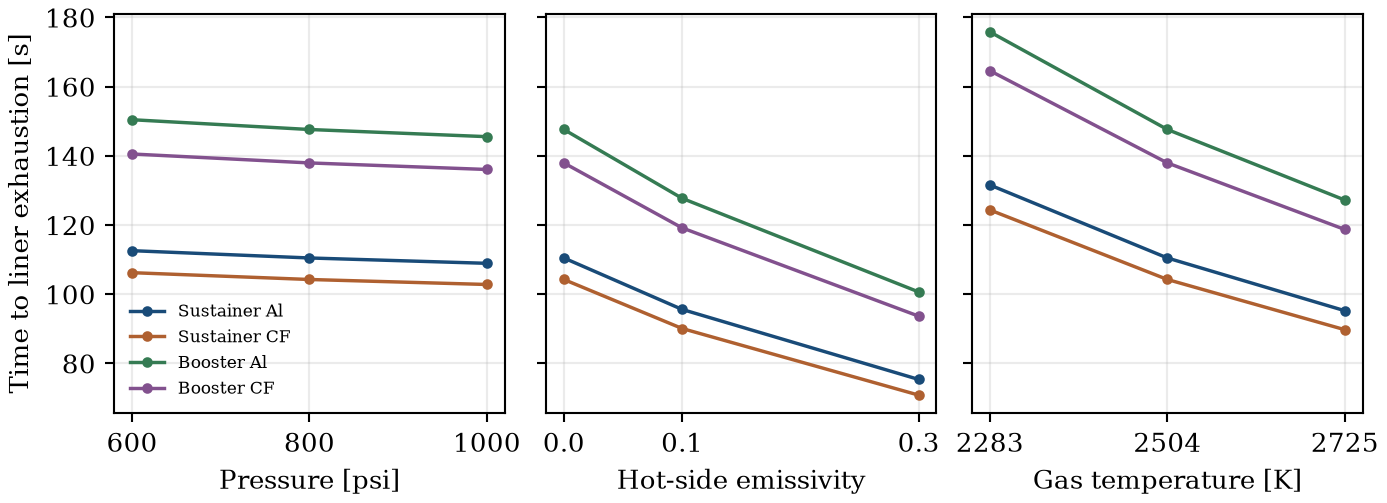
\includegraphics[width=.98\textwidth]{../analysis/evolving_input_sensitivities.png}
\caption{Symbols are separate calculations. A line connects runs with
the other physical inputs fixed. These scenarios do not define a statistical
uncertainty interval.}
\end{figure}
Pressure enters the surface char law. Gas temperature sets the convective
driving temperature. The chosen hot and cold gas scenarios scale the initial
gas-to-wall temperature difference by 1.1 and 0.9 respectively. In the
radiative scenarios, the emitting gas is held at 2504~K. Changing emissivity
also changes the wall temperature, convective heating and exposure duration.
The table gives cumulative radiative energy per original exposed area and
its fraction of total convective plus radiative input.

\begin{center}\small\begin{tabular}{lrrrr}\toprule
&\multicolumn{2}{c}{Emissivity 0.10}&\multicolumn{2}{c}{Emissivity 0.30}\\
Motor & [MJ/m$^2$] & Share [\%]& [MJ/m$^2$] & Share [\%]\\\midrule
Sustainer Al & 20.7 & 15.7 & 48.4 & 36.6 \\
Sustainer CF & 19.4 & 15.8 & 45.2 & 36.9 \\
Booster Al & 27.4 & 15.7 & 64.1 & 36.6 \\
Booster CF & 25.4 & 15.8 & 59.2 & 36.9 \\
\bottomrule\end{tabular}\end{center}
24 of 24 scenarios passed the inventory and separate time-step and mesh checks. Across those runs the largest independent nodal endpoint difference was 0.09~s and the largest sampled thickness difference was 3.6~$\mu$m. The heat load and char chemistry still require measurements on the
actual firing and liner. Each reported endpoint assumes that the casing
keeps its prescribed geometry after its material limit.
\clearpage
